\vspace{-6mm}
\section{}
    \vspace{-3mm}
    \subsection{CODE}
    \vspace{-3mm}
        \subsubsection{client.cc}
            \vspace{-2mm}
            \begin{listing}[h!]
            \inputminted[framerule = 1pt,framesep = 2mm , frame = lines, fontsize=\footnotesize]{c}{./code/week10/Experiment01/client.cpp}
            \vspace{-3mm}
            \caption{\footnotesize experiment 1, client.cc}
            \end{listing}
            \vspace{-6mm}
        \subsubsection{server.cc}
            \vspace{-2mm}
            \begin{listing}[h!]
            \inputminted[framerule = 1pt,framesep = 2mm , frame = lines, fontsize=\footnotesize]{c}{./code/week10/Experiment01/server.cpp}
            \vspace{-3mm}
            \caption{\footnotesize experiment 1, server.cc}
            \end{listing}
            \vspace{-6mm}
\clearpage
    \subsection{SIMULATION RESULTS}
    \vspace{-1mm}
    server / client 두 장치로 무선 네트워크를 구성한다.  simulation 이 시작하면 client 는 server로 메세지를 전송한다.\\
    그 후 server / client는 메세지를 수신했을 경우 서로에게 메세지를 전송하는 동작을 수행한다. 
    \vspace{-3mm}
        \subsubsection{SCREENSHOT}
        시뮬레이션의 결과에서 2개의 모듈 사이에서 메세지의 전송과 재전송을 잘 담기 위해서 화면녹화 screenshot 영상을 촬영해 youtube에 업로드하였다. 해당 영상은 아래의 링크를 클릭해 이동이 가능하다.
        \vspace{-10mm}
            \begin{center}
                \item \href{https://youtu.be/DeSb_LjcU70}
            	{Youtube link of Week10 Experiment 01 Simulation Results Screenshot Video}
            \end{center}
        \vspace{-6mm}
        % 사진 1 2개는 넣어 주자
            \begin{figure}[h!]
            \centering
            \subfloat[Simulation Screenshot 2]{
                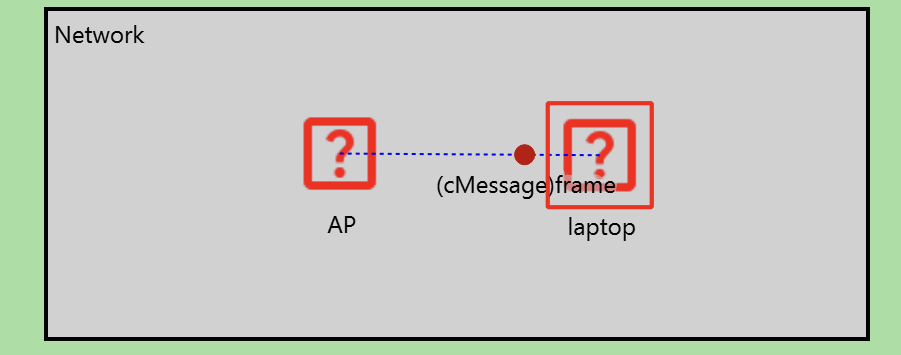
\includegraphics[width=0.48\textwidth]{image/week10/1-1-1.png}
            }\hspace{3mm}
            \subfloat[Simulation Screenshot 2]{
                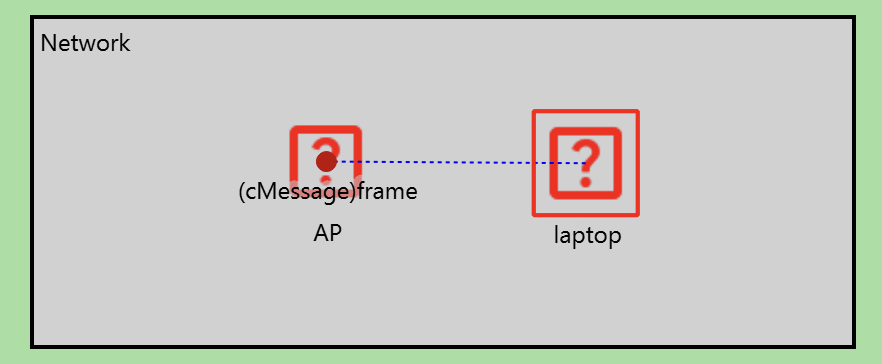
\includegraphics[width=0.46\textwidth]{image/week10/1-1-2.png}
            }
            \caption{Experiment 01 Simulation Results Screenshot}
            \end{figure}
            \vspace{-6mm}
        \subsubsection{RESULTS GRAPH}
            \vspace{-4mm}
            \begin{figure}[!h]\centering 
            	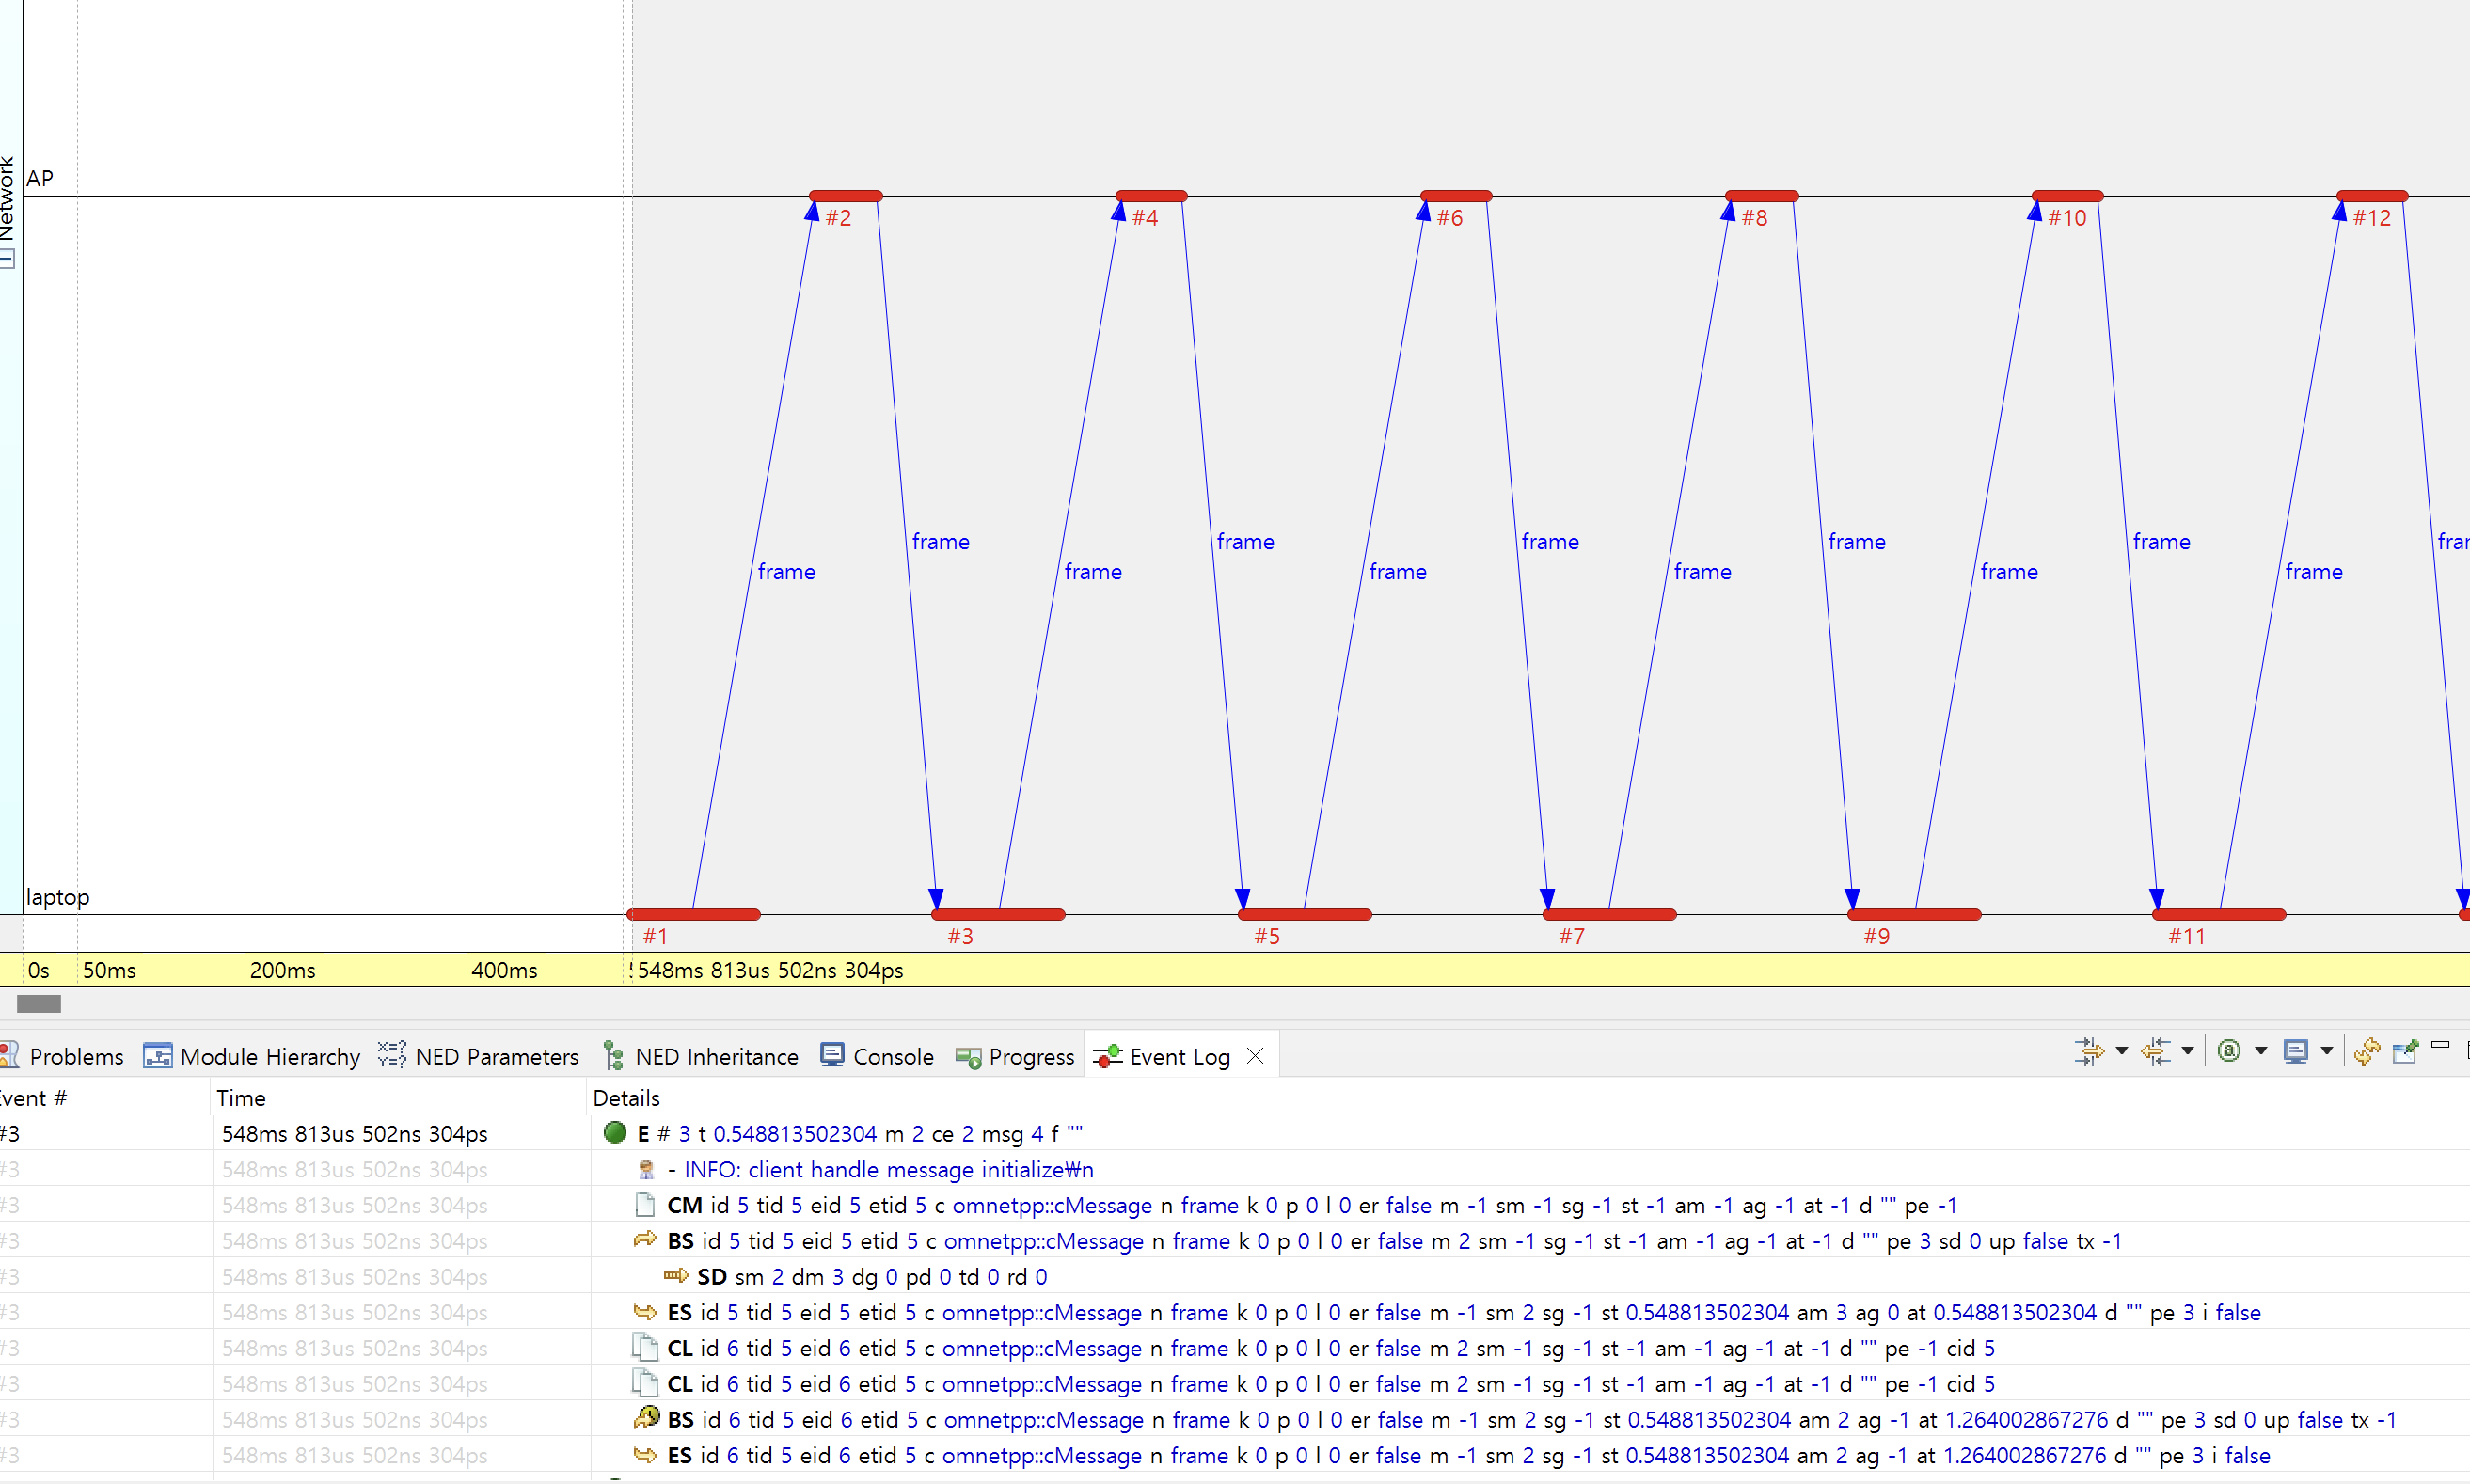
\includegraphics[width=.85\textwidth]{image/week10/1-2.png}
            	\caption{\footnotesize
            	Experiment 01 Simulation Results Sequence Chart}
            	\vspace{-10pt}
            \end{figure}
            \vspace{-4mm}
        \subsubsection{DISCUSSION}
        Exoeriment 1에서는 \mintinline{c}{sendDirect()}를 이용해서 gate를 통하지 않고 송신하고자 하는 module에 직접 msg를 전송하는 무선환경을 가정한 simulation을 진행했다. \mintinline{c}{initialize()}에서 client module 에서 self-msg를 보낸후 \mintinline{c}{handleMessage()}를 통해서 AP에 직접 msg를 전송한다.  이때 무선환경을 가정해 설정해둔 0 $\sim$ 1 사이의 랜덤한 시간에 msg를 보낸다. client, laptop에서 server, AP로 전송된 msg는 server의 \mintinline{c}{handleMessage()}를 통해서 client로 msg를 보내고, 이를 수신한 client의 \mintinline{c}{handleMessage()}에서 다시 반복이 된다.
        
        이렇게 client(laptop) 에서 시작해 server(AP)와 msg를 주고받는 과정을 graph를 통해서 확인할 수 있다. 뿐만아니라 client 에서 msg가 전송되는 시간이 random하게 설정된 부분또한 확인할 수 있다.
\clearpage